\documentclass[crop,tikz,border=3pt,12pt]{standalone}

\usepackage{amsmath}

\newcommand{\tikzsetnextfilename}[1]{}

\definecolor{unitFill}{RGB}{255,255,255}
\definecolor{squareFill}{RGB}{156,201,223}
\definecolor{gridStroke}{RGB}{47,58,69}

\begin{document}
\tikzsetnextfilename{transfer-matrix-tilings-4x2}
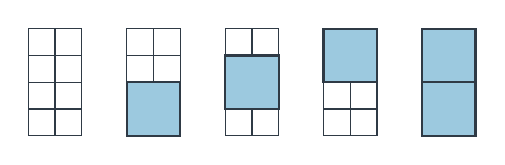
\begin{tikzpicture}[
  x=1cm,
  y=1cm,
  unit/.style={draw=gridStroke, fill=unitFill, line width=0.45pt},
  big/.style={draw=gridStroke, fill=squareFill, line width=0.8pt}
]
  \def\c{0.34}
  \def\g{1.25}

  \foreach \offset in {0,1,2,3,4} {
    \begin{scope}[shift={(\offset*\g,0)}]
      \foreach \x in {0,1} {
        \foreach \y in {0,1,2,3} {
          \path[unit] (\x*\c,\y*\c) rectangle ++(\c,\c);
        }
      }
    \end{scope}
  }

  \begin{scope}[shift={(1*\g,0)}]
    \path[big] (0,0*\c) rectangle ++(2*\c,2*\c);
  \end{scope}

  \begin{scope}[shift={(2*\g,0)}]
    \path[big] (0,1*\c) rectangle ++(2*\c,2*\c);
  \end{scope}

  \begin{scope}[shift={(3*\g,0)}]
    \path[big] (0,2*\c) rectangle ++(2*\c,2*\c);
  \end{scope}

  \begin{scope}[shift={(4*\g,0)}]
    \path[big] (0,0*\c) rectangle ++(2*\c,2*\c);
    \path[big] (0,2*\c) rectangle ++(2*\c,2*\c);
  \end{scope}
\end{tikzpicture}
\end{document}
